\documentclass[acmlarge,nonacm,12pt]{acmart}


%% end of the preamble, start of the body of the document source.
\begin{document}

%%
%% The "title" command has an optional parameter,
%% allowing the author to define a "short title" to be used in page headers.
\title{Sentiment Analysis of Movie Reviews: A Classification Approach for Identifying Positive and Negative Sentiments}

\author{Mounika Gullapalli}
\email{mg7933@missouristate.edu}
\author{Leela Chittoori}
\authornotemark[1]
\email{lc443s@missouristate.edu}
\affiliation{%
  \institution{Missouri State University}
  \city{Springfield}
  \state{Missouri}
  \country{USA}
}

\begin{abstract}
In today’s entertainment landscape, online reviews have become a cornerstone for helping people decide what movies to watch. With the explosion of digital platforms, the sheer volume of these reviews has skyrocketed, making it nearly impossible to manually sift through them all. This project tackles the challenge of automating the process of sentiment analysis for movie ratings. By harnessing the power of machine learning techniques, we aim to develop a system that can categorize user reviews into two simple categories—either "positive" or "negative".

This project explores sentiment analysis of movie reviews using a classification approach. Utilizing the IMDB dataset, we preprocess the data and apply three feature selection methods: Mutual Information, Chi-Square, and Frequency-based feature selection. Employing Naive Bayes classification, we evaluate the performance using key metrics including accuracy, precision, recall, and F1 score. 

Additionally, we visualize the relationship between the number of selected features and F1 score through a plotted graph. Understanding sentiment polarity in movie reviews is crucial for various stakeholders including movie producers, distributors, and viewers. Accurate classification of movie ratings aids in decision-making processes, marketing strategies, and personalized recommendations, ultimately enhancing the overall movie-watching experience and industry performance.


\end{abstract}

\maketitle

\section{Related work}
The field of movie recommendation systems has seen a significant evolution, with researchers exploring various techniques to enhance the accuracy and effectiveness of these systems. This literature review examines the key research papers that have contributed to the development of movie rating classification systems.

One of the early approaches in movie recommendation systems was the analysis of user ratings for movie data classification and recommendation generation. Compared the performance of various classifiers, such as decision trees and support vector machines, in generating movie recommendations based on user ratings. While this approach provided a foundation for movie recommendations. 

Building upon the user rating-based approach, researchers explored the use of traditional statistical methods, such as logistic regression, for generating movie recommendations[9][12][8]. Presented a logistic regression approach for classifying online movie data and generating recommendations based on user reviews. This method provided a more nuanced understanding of user preferences.

The integration of sentiment analysis into movie recommendation systems has been a significant focus of recent research. Proposed a movie recommendation system that incorporates sentimental analysis using the cosine similarity technique[1], demonstrating the benefits of considering user sentiment in the recommendation process. Similarly, explored the use of natural language processing (NLP) tools to analyze movie reviews and incorporate sentiment information into the recommendation system[2].

Expanding the scope of sentiment analysis, presented a study on sentiment analysis of Tamil tweets using deep convolutional neural networks[3], showcasing the potential of advanced machine learning techniques in sentiment extraction. This work highlighted the broader applicability of sentiment analysis beyond the movie domain.

While the aforementioned studies focused on sentiment analysis, researchers have also explored the use of machine learning and deep learning techniques for movie recommendation systems[3][4]. investigated the use of a machine learning approach for sentiment analysis of movie reviews, while focused on summarizing and performing sentiment analysis on movie critics’ data[5].

The comparative performance of different deep learning techniques for sentiment analysis was examined in providing insights into the strengths and limitations of various models. This work laid the foundation for more advanced sentiment analysis techniques in recommendation systems[6]. Expanding beyond movies, explored the extraction of gamers’ opinions from reviews[7], demonstrating the broader applicability of sentiment analysis techniques across different domains.

More recently, researchers have explored the integration of deep learning techniques with recommendation systems. This paper proposed a convolutional recommended neural network system based on user reviews for movies, showcasing the potential of deep learning in enhancing recommendation accuracy[10]. 

The sentiment analysis and classification of movie reviews were further explored in, high- lighting the importance of sentiment information in movie recommendation systems[11][13]. Building on this, presented a study on movie success prediction using machine learning techniques, demonstrating the potential of incorporating additional factors beyond sentiment analysis.

Finally, a systematic analysis of movie recommendation systems was conducted through sentiment analysis, providing a comprehensive overview of the field and identifying future research directions.


Overall, this literature review highlights the evolution of movie recommendation systems, starting from the basic user rating-based approaches and progressing towards the more advanced techniques that incorporate sentiment analysis and deep learning. Also, explained how the classification techniques were implemented as a part of recommendation systems. The research papers discussed in this review showcase the significant advancements in the field and the potential for further improvements in the accuracy and personalization of movie recommendations.

\section{Proposed Method}

The "IMDB" dataset has been used to implement this project and the pre-processing phase begins with the removal of HTML tags from the raw movie reviews using regular expressions. Following this, special characters are eliminated from the text to enhance readability and facilitate subsequent analysis. Moreover, non-ASCII characters are filtered out to ensure compatibility with downstream processing steps.

Numerical digits are then removed from the text using regular expressions, as they often do not contribute significantly to sentiment analysis and may introduce noise. Subsequently, the text is tokenized into individual words using NLTK's `word tokenize` function, breaking it down into manageable units for further processing.To standardize the text, all words are converted to lowercase, ensuring uniformity in the dataset and mitigating the impact of case sensitivity on model performance. Stopwords, common words that do not carry significant meaning, are then removed from the tokenized text using a predefined list. This step helps focus the analysis on meaningful content while reducing noise.

Stemming is applied to further refine the text by reducing words to their root form, thereby consolidating semantically similar terms. The Porter Stemmer algorithm, provided by NLTK, is employed for this purpose. By applying these preprocessing techniques, the raw movie reviews are transformed into a clean and standardized format suitable for feature extraction and sentiment analysis.Following data preprocessing, feature engineering was conducted using TF-IDF vectorization. 

This process transformed the preprocessed text into numerical vectors, assigning each word a weight reflecting its importance in the dataset. Subsequently, feature selection techniques were applied to identify the most relevant features for analysis. Mutual Information and Chi-Square methods, implemented through SelectKBest, were utilized to select features based on their correlation with the target variable. Furthermore, a frequency-based approach was employed to choose the most common terms in the dataset as features.

With the feature selection completed, the Naive Bayes classification algorithm was employed on those obtained features for model training and evaluation. The Naive Bayes class was customized to calculate prior and conditional probabilities for each class, facilitating efficient prediction of sentiment labels. Model performance was assessed using standard evaluation metrics, including accuracy, precision, recall, and F1 score. Additionally, a systematic experimentation was conducted to explore the impact of varying the number of selected features on model performance.To provide a visual representation of the experimental results, a line graph was generated to illustrate the relationship between the number of selected features and the F1 score for each feature selection method. This visualization aided in understanding the trade-off between feature dimensionality and model effectiveness. Through this comprehensive methodology, the project aimed to develop a robust sentiment analysis system for classifying movie reviews into positive and negative sentiments.

\section{Results}

\textbf{Mutual Information Feature Selection}

From the Fig. 1, we can observe the Evaluation metrics of Mutual Information Feature Selection i.e., Accuracy, Precision, Recall and F1-score.

\begin{figure}[h]
    \centering
    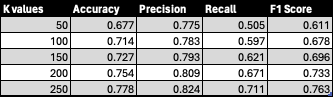
\includegraphics[width=1\linewidth]{Mutual_all_metrics.png}
    \caption{Accuracy, Precision, Recall and F1-Score for different k values using Mutual Information Feature Selection}
    \label{fig:enter-label}
\end{figure}
\textbf{Chi-Square Feature Selection}

From the Fig. 2, we can observe the Evaluation metrics of Chi-Square Feature Selection i.e., Accuracy, Precision, Recall and F1-score.

\begin{figure}[h]
    \centering
    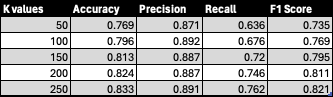
\includegraphics[width=1\linewidth]{Chi_all_metrics.png}
    \caption{Accuracy, Precision, Recall and F1-Score for different k values using Chi-Square Feature Selection}
    \label{fig:enter-label}
\end{figure}


\textbf{Frequency-based Feature Selection}

From the Fig. 3, we can observe the Evaluation metrics of Frequency-based Feature Selection like Accuracy, Precision, Recall and F1-score.


\begin{figure}[h]
    \centering
    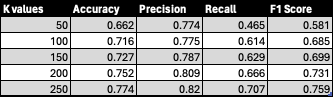
\includegraphics[width=1\linewidth]{Frequency_all_metrics.png}
    \caption{Accuracy, Precision, Recall and F1-Score for different k values using Frequency-based Feature Selection}
    \label{fig:enter-label}
\end{figure}



The project's evaluation of three distinct feature selection methods—Mutual Information, Chi-Square, and Frequency-based selection—across varying numbers of selected features is presented in Figures 1, 2, and 3. Despite generating accuracy, precision, and recall metrics, F1-score emerges as the preferred evaluation metric due to its comprehensive assessment of model performance by considering both false positives and false negatives. This preference is reinforced by Figure 5, a graph generated by considering values from Fig. 4, visually depicts the F1 Scores plotted against the number of features for each method, facilitating a clear understanding of performance trends. Moreover, this graph underscores the importance of selecting an appropriate feature selection method and aids in determining the optimal K value for the selected method. Such insights are instrumental in refining model performance and guiding further investigation into feature selection methods to optimize predictive accuracy and robustness.

\begin{figure}
    \centering
    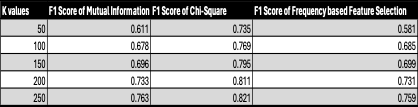
\includegraphics[width=1\linewidth]{F1vsk.png}
    \caption{K value vs Cumulative F1 score for all the 3 feature selection methods}
    \label{fig:enter-label}
\end{figure}


\begin{figure}[h]
    \centering
    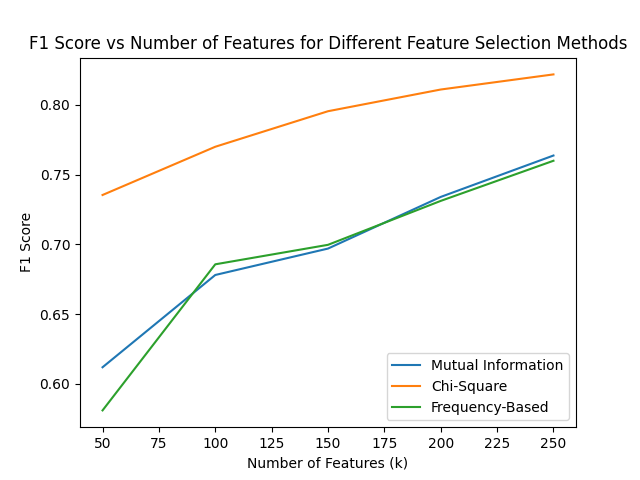
\includegraphics[width=\linewidth]{50_100_150_200_250.png}
    \caption{Graph Representing the Number of Features vs F1-Score}
    \label{fig:enter-label}
\end{figure}


\section{Analysis}

Below are the notable analyses derived from the evaluation metrics of all the 3 feature selection methods:

\begin{itemize}
    \item \textbf{Performance Improvement with Increasing K values: }Across all three feature selection methods, as the number of selected features (K values) increases, there is a general trend of improvement in performance metrics (accuracy, precision, recall, and F1 score). This indicates that including more relevant features tends to enhance the model's predictive ability.
    \item \textbf{Chi-Square Feature Selection Shows Superior Performance: }Among the three methods, Chi-Square feature selection consistently yields the highest performance across all metrics and K values. It consistently achieves the highest accuracy, precision, recall, and F1 score compared to Mutual Information and Frequency-based feature selection. This suggests that Chi-Square feature selection might be more effective in identifying discriminative features for the given classification task.
    \item \textbf{Mutual Information and Frequency-based Selection Performances:} While Mutual Information and Frequency-based feature selection methods exhibit similar trends in performance, they consistently fall slightly behind Chi-Square feature selection. 
    \item \textbf{Execution Time:} We have utilized the Python packages 'cProfile' and 'pstats' for profiling and analyzing the execution time of our code. These packages enabled detailed examination of the runtime behavior of the function sin my code. The profiling analysis indicates that the feature selection process, particularly using mutual information, consumes the majority of execution time due to computations within the mutual\_info\_classif function and its internal functions (\_compute\_mi and \_estimate\_mi). This suggests that optimizing the mutual information-based feature selection step could significantly improve overall performance.
\end{itemize}


The graph in Fig. 5, confirms our earlier analysis, demonstrating that Chi-Square Feature Selection consistently outperforms Mutual Information and Frequency-based methods across varying numbers of features. This alignment between the graph and our previous metrics analysis validates the superiority of Chi-Square in selecting discriminative features for the classification task.

\section{Conclusion}

In today's digital world, where movie choices are abundant, analyzing reviews has become essential for viewers to decide what to watch. This project aimed to automate this process using Naive Bayes Classification Algorithm. By sorting reviews into "positive" or "negative" categories, it helps people quickly understand the general review about a movie. The study experimented with different techniques to improve performance metrics, finding that Chi-Square feature selection consistently performed best. This suggests that certain words or phrases carry more weight in determining whether a review is positive or negative and Chi-Square does a great job in finding the right words for correctly classifying the reviews.

Furthermore, the research highlighted a notable finding regarding the computational efficiency of feature selection methods. Mutual Information feature selection, while effective in some aspects, was observed to consume a significant amount of time during the analysis. This suggests that optimizing the mutual information-based feature selection step could greatly enhance overall performance. 

Overall, this research shows promise in making movie-watching decisions easier for everyone involved. From producers to viewers, understanding sentiment helps in making better choices, improving marketing strategies, and enhancing the overall movie experience. By leveraging machine learning techniques, the project offers a systematic approach to sentiment analysis, paving the way for more accurate and efficient movie recommendation systems in the future.

\bibliographystyle{ACM-Reference-Format}

\bibliography{sample-base}
[1] A. Javed, F. Rehman, N. Sarfraz, H. Sharif, R. Khan and A. M. Khan, "Movie Recommendation System with Sentimental Analysis Using Cosine Similarity Technique," 2022 3rd International Conference on Innovations in Computer Science \& Software Engineering (ICON- ICS), Karachi, Pakistan, 2022, pp. 1-8, doi:  10.1109/ICONICS56716.2022.10100512.

[2] N. Kapoor, S. Vishal and K. K. S., "Movie Recommendation System Using NLP Tools," 2020 5th International Conference on Communication and Electronics Systems (ICCES), Coimbatore, India, 2020, pp. 883-888, doi: 10.1109/ICCES48766.2020.9137993.

[3] M. Rajasekar and A. Geetha, "Sentiment Analysis of Tamil Tweets Using Deep Con- volution Neural Networks," 2023 First International Conference on Advances in Electrical, Electronics and Computational Intelligence (ICAEECI), Tiruchengode, India, 2023, pp. 1-5, doi: 10.1109/ICAEECI58247.2023.10370847.

[4] M. T. Zumma, K. B. M. Tahmiduzzaman, R. Khan, N. S. Roni, A. A. M. Rahat-Bin-Rafique and A. H. Akash, "Sentimental Analysis of Movie Review using Machine Learning Approach," 2022 IEEE International Conference on Current Development in Engineering and Technology (CCET), Bhopal, India, 2022, pp. 1-5, doi: 10.1109/CCET56606.2022.10080860.

[5] S. S. Vavilapalli, P. ReddyKorepu, S. Saggam, M. Pentyala and S. A. Devi, "Summarizing \& Sentiment Analysis on Movie Critics Data," 2021 6th International Conference on Inventive Computation Technologies (ICICT), Coimbatore, India, 2021, pp. 1-5,

doi: 10.1109/ICICT50816.2021.9358563.

[6] R. G. Tiwari, A. Misra and N. Ujjwal, "Comparative Classification Performance Evalu- ation of Various Deep Learning Techniques for Sentiment Analysis," 2022 8th International Conference on Signal Processing and Communication (ICSC), Noida, India, 2022, pp. 304-309, doi: 10.1109/ICSC56524.2022.10009471.

[7] D. Sirbu, A. Secui, M. Dascalu, S. A. Crossley, S. Ruseti and S. Trausan-Matu, "Extracting Gamers’ Opinions from Reviews," 2016 18th International Symposium on Symbolic and Numeric Algorithms for Scientific Computing (SYNASC), Timisoara, Romania, 2016, pp. 227-232, doi: 10.1109/SYNASC.2016.044.

[8] A. Benlahbib, A. Boumhidi and E. H. Nfaoui, "A Logistic Regression Approach for Gener- ating Movies Reputation Based on Mining User Reviews," 2019 International Conference on Intelligent Systems and Advanced Computing Sciences (ISACS), Taza, Morocco, 2019, pp. 1-7, doi: 10.1109/ISACS48493.2019.9068916.

[9] Jyoti, S. Dhawan and K. Singh, "Analysing user ratings for classifying online movie data using various classifiers to generate recommendations," 2015 International Conference on Futuristic Trends on Computational Analysis and Knowledge Management (ABLAZE), Greater Noida, India, 2015, pp. 295-300, doi: 10.1109/ABLAZE.2015.7155014.

[10] P. Kirubanantham, A. Saranya and D. S. Kumar, "Convolutional Recommended Neural Network system based on user reviews for movies," 2021 4th International Conference on Computing and Communications Technologies (ICCCT), Chennai, India, 2021, pp. 17-21, doi: 10.1109/ICCCT53315.2021.9711772.

[11] M. Yasen and S. Tedmori, "Movies Reviews Sentiment Analysis and Classification," 2019 IEEE Jordan International Joint Conference on Electrical Engineering and Information Technology (JEEIT), Amman, Jordan, 2019, pp. 860-865, doi: 10.1109/JEEIT.2019.8717422.

[12] N. Darapaneni et al., "Movie Success Prediction Using ML," 2020 11th IEEE Annual Ubiquitous Computing, Electronics \& Mobile Communication Conference (UEMCON), New York, NY, USA, 2020, pp. 0869-0874, doi: 10.1109/UEMCON51285.2020.9298145.

[13] R. Lavanya and B. Bharathi, "Systematic analysis of Movie Recommendation System through Sentiment Analysis," 2021 International Conference on Artificial Intelligence and Smart Systems (ICAIS), Coimbatore, India, 2021, pp. 614-620, doi: 10.1109/ICAIS50930.2021.9395854.
\end{document}
